\documentclass[12pt,letterpaper,oneside]{report}

%---------------------PACKAGES
\usepackage[margin=3cm]{geometry}
\usepackage[utf8]{inputenc}
\usepackage{graphicx}
\usepackage[spanish]{babel}
\usepackage[fixlanguage]{babelbib}
\selectbiblanguage{spanish}
\usepackage{url}
\usepackage{float}
%-----------------------------

\title{Trust Me}
\author{{Brayan Arango} \\ {Wilder Alcala}}

%-----------------CONFIG
\renewcommand{\labelitemi}{$\bullet$}
\renewcommand{\labelitemii}{$-$}
\setcounter{tocdepth}{4}
\setcounter{secnumdepth}{4}
%-----------------------

\begin{document}
	
	%-----------------INDEX
	\begin{titlepage}
	\begin{center}
	\textbf{DISEÑO DE UN PROTOTIPO DE PLATAFORMA WEB, QUE PERMITA LA GESTIÓN DE MICROCRÉDITOS ENTRE SUS USUARIOS.}\\
	\vspace{5cm}
	
	{WILDER MANUEL ALCALÁ VIZCAINO}\\
	{BRAYAN CAMILO ARANGO RIVERA}\\ 
	\vspace{4cm}
	
	
\includegraphics[width=0.4\textwidth]{start/Universidad}\\
	\vspace{0.5cm}
	
	{UNIVERSIDAD DISTRITAL FRANCISCO JOSÉ DE CALDAS}\\
	{FACULTAD DE INGENIERÍA}\\
	{ESPECIALIZACIÓN EN INGENIERÍA DE SOFTWARE}\\
	{BOGOTÁ D.C, COLOMBIA}\\
	{2019}\\
	\end{center}
\end{titlepage}
	\begin{titlepage}
	\begin{center}
	\textbf{DESARROLLO DE UN PROTOTIPO DE PLATAFORMA WEB, QUE PERMITA LA GESTIÓN DE MICROCRÉDITOS ENTRE SUS USUARIOS.}\\
	\vspace{2.5cm}
	
	\textbf{AUTORES:}\\
	{WILDER MANUEL ALCALÁ VIZCAINO}\\
	{BRAYAN CAMILO ARANGO RIVERA}\\ 
	\vspace{2.5cm}
	
	{PROYECTO DE GRADO PRESENTADO PARA OPTAR POR EL TÍTULO DE ESPECIALISTA EN INGENIERÍA DE SOFTWARE.}\\
	\vspace{2.5cm}
	
	\textbf{DIRECTORA:}\\
	{ALEXANDRA ABUCHAR PORRAS}\\
	\vspace{1cm}
	
	\textbf{REVISOR:}\\
	{ALEJANDRO PAOLO DAZA CORREDOR}\\
	\vspace{2cm}
	

	
	
	{UNIVERSIDAD DISTRITAL FRANCISCO JOSÉ DE CALDAS}\\
	{FACULTAD DE INGENIERÍA}\\
	{ESPECIALIZACIÓN EN INGENIERÍA DE SOFTWARE}\\
	{BOGOTÁ D.C, COLOMBIA}\\
	{2019}\\
	\end{center}
\end{titlepage}

	\pagenumbering{Roman}
	\urlstyle{same}
	\begin{flushright}
	\textbf{Nota de aceptación}\\
	\vspace{1cm}
	
	\rule{5cm}{0.1mm}\\
	\rule{5cm}{0.1mm}\\
	\rule{5cm}{0.1mm}\\
	\rule{5cm}{0.1mm}\\
	\rule{5cm}{0.1mm}\\
	\rule{5cm}{0.1mm}\\
	\rule{5cm}{0.1mm}\\
	\vspace{3cm}
	
	
	\rule{5cm}{0.1mm}\\
	\textbf{Decano}\\
	\vspace{2.5cm}
	
	\rule{5cm}{0.1mm}\\
	\textbf{Director}\\
	\vspace{2.5cm}
	
	\rule{5cm}{0.1mm}\\
	\textbf{Revisor}\\
	\vspace{2.5cm}
	
	\flushleft \textbf{ Bogotá, D.C 2019}
	
\end{flushright}
	\chapter*{\flushright Dedicatoria}

\begin{flushright}
	\textit{Dedicado a nuestras familias, las cuales han sacrificado \\ su tiempo de compartir con nosotros, por nuestro saber.}
\end{flushright}
	
	%--------------------TABLES
	\tableofcontents
	\listoffigures
	%\listoftables
	
	%-----------------CONTENT
	\addcontentsline{toc}{part}{INTRODUCCION}
\pagenumbering{arabic}
\chapter*{INTRODUCCION}

\textit{Dedicado a nuestras familias, las cuales han sacrificado tiempo para compartir con nosotros, por nuestro saber.}
	
	\part{CONTEXTUALIZACIÓN DE LA INVESTIGACIÓN}
	
		\chapter{DESCRIPCION DE LA INVESTIGACIÓN}
			\section{Estudio del problema de investigación}

	\subsection{Planteamiento del Problema}
	
	{Las entidades bancarias en Colombia, son los entes principales en gestionar créditos para sus clientes, estas se encargan de ofrecer créditos según el perfil de la persona interesada, tomando en cuenta, sus ingresos, la capacidad de endeudamiento y los reportes en las centrales de riesgo, limitando así, el acceso de personas con ingresos bajos y sin vida crediticia, a este tipo de beneficio \cite{bankrep}. Incluso, en algunos casos, el monto del crédito requerido por el usuario es tan bajo, que no amerita el tramite necesario para acceder a él, obligando a la persona a afrontar necesidades básicas las cuales no puede suplir en el momento.\\
		
	A esto se le suma, el aumento de la tasa desempleo que para este año según cifras DANE va en un 10,8\%, aumentando un 1,6\% con respecto al año pasado que estaba en un 9.2\% \cite{dane}, esto gracias, al alto crecimiento de la población \cite{unemployment}, si bien la crisis económica del vecino país Venezuela, ha obligado a gran parte de sus habitantes a migrar hacia Colombia, estos por la falta de empleo y necesidad,  ofrecen sus servicios profesionales a menores rangos salariales,  influyendo en la estabilidad y el bolsillo de los colombianos.\\
	
	Frente a esta problemática y las necesidades expuestas, un grupo de personas que trabajan en la informalidad, como vendedores ambulantes e incluso tenderos, buscando subsanar el alto índice de intereses cobrado por las entidades bancarias, ofrecen sus productos a clientes de confianza con módicas cuotas de pago, facilitándoles el acceso a recursos básicos de bajo costo, los cuales, una entidad financiera normalmente no financiaría, dicho procedimiento es conocido como “fiar”, en otros términos, ofrecer un microcrédito, donde el tendero usualmente toma registro de cada ítem fiado en una agenda o cuaderno, permitiendo fácilmente la manipulación, ingreso errado (malos cálculos) y la perdida, de la información, pues el registro estará supeditado al tendero, conllevando a un alto grado de incertidumbre en el cliente representado en molestar.\\

	Por otro lado, también existe una problemática relacionada en cuanto a préstamos entre conocidos se refiere, pues algunas personas son amantes de las apuestas y a veces se ven envueltos en deudas con sus conocidos por estas, o por causas de fuerza mayor que los obligan a pedir un préstamo de dinero, y es allí donde se presenta la falencia, pues al ser un proceso irrelevante para ellos (por ser de confianza), no toman registro de la transacción o hacen una simple anotación en cuadernos, celulares, agendas etc, permitiendo que la transacción quede en el olvido o se pierda.}

	\subsection{Formulación del problema}
	
	{Con base a la problemática anterior expuesta, surge la siguiente pregunta de investigación ¿Cómo facilitar la gestión de microcréditos entre el tendero, consumidor o personas naturales por medio de una plataforma WEB?.}
	
	\subsection{Sistematización del problema}
	
	{¿Bajo qué fórmulas se rigen las entidades financieras para el cálculo de cuotas, en caso de un usuario pagar a plazos?.\\
		
	¿Cómo permitir el fácil acceso a la información de los microcréditos obtenidos por él consumidor, ante él tendero?.\\
	
	¿Cómo conservar indefinidamente la información de los microcréditos, sin que esta se pierda por manipulación del usuario?.}
			\section{Objetivos}

	\subsection{Objetivo general}
	
	{Desarrollar un prototipo de plataforma WEB, que permita la gestión de microcréditos entre sus usuarios, con el fin de facilitar el cálculo y visualización de estos en una interfaz amigable.}
	
	\subsection{Objetivos específicos}
	
	\begin{itemize}
		\renewcommand{\labelitemi}{$\bullet$}
		\item Aumentar las ventas de los tenderos en un 10\% al basar su sistema de microcréditos en la plataforma WEB.
		\item Eliminar la incertidumbre del cliente con respecto a los microcréditos obtenidos ante el tendero.
		\item Reducir el uso desmesurado de microcréditos por parte del consumidor, con la limitación de estos, para un mejor manejo de sus finanzas.
	\end{itemize}
	
	
	
	
	
	
			\section{Justificacion}
			\section{Alcances y limitaciones}
			\section{Hipótesis}

{Dado los avances tecnológicos y el gran acogimiento que este ha tenido en la actualidad, el desarrollo de una plataforma web para el transporte y recepción de ítems únicos por región, logrará acortar las barreras regionales entre los usuarios y permitirá el libre flujo mercancía a bajos costos.}
			\section{Marco referencial}

	\subsection{Marco teórico}
	
		\subsubsection{Sitios Web}
		
		{Un sitio web es un conjunto de archivos electrónicos y páginas web referentes a un tema en particular, incluyendo una página inicial de bienvenida generalmente denominada home page, a los cuales se puede acceder a través de un nombre de dominio y dirección en Internet específicos. El World Wide Web, o simplemente Web como se le llama comúnmente, está integrado por sitios web y éstos a su vez por páginas web. La gente suele confundir estos términos, pero un sitio web es en realidad un conjunto de páginas web .\\
			
		Los sitios web son empleados por las instituciones públicas y privadas, organizaciones e individuos para comunicarse con el mundo entero. En el caso particular de las empresas, este mensaje tiene que ver con la oferta de sus bienes y servicios a través de Internet, y en general para hacer eficiente sus funciones de mercadotecnia.}
	
	
		\subsubsection{Diseño Web responsivo}
		
		{El diseño web responsive o adaptativo es una técnica de diseño web que busca la correcta visualización de una misma página en distintos dispositivos. Desde ordenadores de escritorio a tablets y móviles, en otras palabras, se trata de redimensionar y colocar los elementos de la web de forma que se adapten al ancho de cada dispositivo permitiendo una correcta visualización y una mejor experiencia de usuario. Se caracteriza porque los layouts (contenidos) e imágenes son fluidos y se usa código media-queries de CSS3.\\
			
		El diseño responsive permite reducir el tiempo de desarrollo, evita los contenidos duplicados, y aumenta la viralidad de los contenidos ya que permite compartirlos de una forma mucho más rápida y natural.}
	
	
		\subsubsection{Bases de datos relaciones}
		
		{Una base de datos relacional consiste en un conjunto de tablas, a cada una de las cuales se le asigna un nombre exclusivo, cada fila de la tabla representa una relación entre un conjunto de valores. De manera informal, cada tabla es un conjunto de entidades, y cada fila es una entidad, dado que cada tabla es un conjunto de tales relaciones, hay una fuerte correspondencia entre el concepto de tabla y el concepto matemático de relación, del que toma su nombre el modelo de datos relacional.}
		
	
	\subsection{Marco Conceptual}
	
		\subsubsection{SQL}
		
		{El álgebra relacional proporciona una notación concisa y formal para la representación de las consultas. Sin embargo, los sistemas de bases de datos comerciales necesitan un lenguaje de consultas más cómodo para el usuario. SQL es un lenguaje de consultas distribuido comercialmente de más influencia. SQL usa una combinación de constructores del álgebra relacional y del cálculo relacional.\\
			
		Aunque se haga referencia al lenguaje SQL como “lenguaje de consultas”, puede hacer mucho más que consultar las bases de datos. Usando SQL es posible además definir la estructura de los datos, modificar los datos de la base de datos y especificar restricciones de seguridad.\\
	
		No se pretende proporcionar un manual de usuario completo de SQL. En cambio, se presentan los constructores y conceptos fundamentales de SQL. Las distintas implementaciones de SQL pueden diferenciarse en detalles o admitir sólo un subconjunto del lenguaje completo.}
	
	
		\subsubsection{RESTful}
		
		{La Transferencia de Estado Representacional (REST - Representational State Transfer) fue ganando amplia adopción en toda la web como una alternativa más simple a SOAP y a los servicios web basados en el lenguaje de descripción de servicios Web (Web Services Descripcion Language - WSDL). Ya varios grandes proveedores de Web 2.0 están migrando a esta tecnología, incluyendo a Yahoo, Google y Facebook, quienes marcaron como obsoletos a sus servicios SOAP y WSDL y pasaron a usar un modelo más fácil de usar, orientado a los recursos.\\
			
		REST define un set de principios arquitectónicos por los cuales se diseñan servicios web haciendo foco en los recursos del sistema, incluyendo cómo se accede al estado de dichos recursos y cómo se transfieren por HTTP hacia clientes escritos en diversos lenguajes. REST emergió en los últimos años como el modelo predominante para el diseño de servicios. De hecho, REST logró un impacto tan grande en la web que prácticamente logró desplazar a SOAP y las interfaces basadas en WSDL por tener un estilo bastante más simple de usar.}
	
	
		\subsubsection{Web api}
		
		{Es un marco que facilita la creación de servicios HTTP disponibles para una amplia variedad de clientes, entre los que se incluyen exploradores y dispositivos móviles. ASP.NET Web API es la plataforma perfecta para crear aplicaciones RESTful en .NET Framework.}
		
		
		\subsubsection{HTTP}
		
		{Hypertext Transfer Protocol (HTTP) (o Protocolo de Transferencia de Hipertexto en español) es un protocolo de la capa de aplicación para la transmisión de documentos hipermedia, como HTML. Fue diseñado para la comunicación entre los navegadores y servidores web, aunque puede ser utilizado para otros propósitos también. Sigue el clásico modelo cliente-servidor, en el que un cliente establece una conexión, realizando una petición a un servidor y espera una respuesta del mismo. Se trata de un protocolo sin estado, lo que significa que el servidor no guarda ningún dato (estado) entre dos peticiones. Aunque en la mayoría de casos se basa en una conexión del tipo TCP/IP, puede ser usado sobre cualquier capa de transporte segura o de confianza, es decir, sobre cualquier protocolo que no pierda mensajes silenciosamente, tal como UDP.}
		
		
		\subsubsection{Modelo Cliente - Servidor}
		
		{Modelo de diseño de software en el que las tareas se reparten entre los proveedores de recursos o servicios, llamados servidores, y los demandantes, llamados clientes. Un cliente realiza peticiones a otro programa, el servidor, quien le da respuesta.}
	
	
		\subsubsection{Arquitectura Orientada a Servicios SOA}
		
		{Modelo de diseño de software en el que las tareas se reparten entre los proveedores de recursos o servicios, llamados servidores, y los demandantes, llamados clientes. Un cliente realiza peticiones a otro programa, el servidor, quien le da respuesta.}
			\section{Metodología de la investigación}

	\subsection{Tipo de estudio}
	
	{Dado el tema de investigación, el tipo de estudio a realizar se enmarca dentro del tipo descriptivo, el cual, pretende dar una descripción del objeto de estudio, especificando sus propiedades o atributos más relevantes, para así, fortalecer la justificación del porqué el desarrollo del proyecto, se acudirá a la implementación de técnicas de recolección de información, basadas en la observación, entrevistas y/o cuestionarios, permitiendo la identificación de la tendencia actualmente de las personas, por utilizar plastaformas para alcanzar o conseguir un bien común, tal como se evidencia en plataformas populares como uber, uber eats, rappi, etc.}
	
	
	\subsection{Método de investigación}
	
	{El método a implementar en este estudio investigativo, es el de la observación, el cual, permitirá obtener conocimiento acerca del fenómeno presentado actualmente dentro de las comunidades que emplean medios tecnológicos, se enfoca en observar para obtener información del problema, estimulando la curiosidad e impulsando al desarrollo de nuevos hechos de interés científico, es ideal, para el tipo de estudio planteado, ya que se puede complementar con la utilización de otros procedimientos o técnicas propuestos, como lo son entrevistas y cuestionarios, permitiendo la comparación de los resultados recogidos y obtener una información más precisa, haciendo posible investigar el fenómeno tecnológico directamente}
	
	
	\subsection{Fuentes y técnicas para la recolección de la información}
	
	{Para la recolección de información nos basaremos en las fuentes primarias, las cuales, serían los usuarios de tecnologías orientadas a comunidades, como usuarios de Uber, rappi, etc, de ellos, obtendremos la información directa por medio de las técnicas antes mencionadas:
		
	\begin{itemize}
		\item Encuestas: se realiza el registro de situaciones que puedan ser observadas y en ausencia de poder ser recreado un experimento se cuestiona al participante sobre ello.
		
		\item Experimentación: Se manipulan las variables que rodean la problemática, permitiendo analizar los efectos causados por estos y verificar si las diferencias obtenidas son significativas.
	\end{itemize}
		
	Adicionalmente, se obtendrá información de fuentes secundarias como lo son documentos de internet o medios de comunicación, siempre y cuando, la información sea pertinente y fidedigna.}
	
	\subsection{Tratamiento de la información}
	
	{Se realizará un análisis cualitativo de la información obtenida, realizando una conversión de esta y garantizando una mirada crítica para filtrar la información que constituirá la fuente principal de la investigación, desligando de datos complementarios, que también serán útiles para el desarrollo del proyecto.}
			
	\part{DESARROLLO DE LA INVESTIGACIÓN}

		\chapter{ORGANIZACIÓN}
			\section{Introducción}

{En este capítulo se le da un enfoque de negocio al proyecto de grado, se le concede un nombre comercial en inglés “Tru\$tMe”, el cual traducido al español significa confíame, se estable una estructura organizacional que aborda los aspectos empresariales del proyecto.}
			\section{Tru\$tMe}

{Es una empresa colombiana dedica a la gestión de préstamos o “fios” entre sus usuarios, esta permite que la persona que ingrese con un rol de tendero, pueda ofertar sus productos y quienes estén interesados (conocidos del tendero) acceder a los mismos con facilidades de pago, como lo es el pago a cuotas.}
			\section{Misión}

{Ser la empresa líder colombiana en la gestión de préstamos entre sus usuarios, permitiendo el aumento de las ventas de las personas que confíen en la app como herramienta para vender sus productos y brindando transacciones confiables a sus clientes.}
			\section{Visión}

{Influir en la economía de los principales almacenes de cadena de Colombia, como herramienta de gestión de créditos, permitiendo aumentar la clientela objetivo y aportar al crecimiento económico de los colombianos de bajos recursos.}
			\section{Objetivos operativos}

\begin{itemize}
	\item Controlar los préstamos realizados por los tenderos a sus clientes, con la ayuda  de una interfaz amigable.
	\item Brindar acceso a las personas de bajos recursos, a productos de la canasta familiar, con facilidades de pago.
	\item Permitir a las personas naturales prestar dinero a sus conocidos, sin riesgo de perder la información del préstamo.
\end{itemize}
			\section{Principios fundadores}

\begin{itemize}
	
	\item Las entidades colombianas, quienes limitan a las personas de bajos recursos a acceder a una vida digna, con la adquisición de productos de bajo costo que suplan sus necesidades básicas, no están cumpliendo con los principios de igualdad y le están negando el desarrollo económico como persona y ciudadano, a quien lo necesita.
	
	\item Para un mejor desarrollo y sostenibilidad económica, se les debe facilitar el acceso a herramientas tecnológicas, a las personas quienes con tanto esfuerzo han logrado surgir con pequeños negocios, ayudándolos a competir con grandes empresas en igualdad de condiciones.
	
\end{itemize}
			\section{Servicios}

{Los principales servicios que ofrece la aplicación web son los siguientes:

\begin{itemize}
	\item Pagos de deudas.
	\item Pedir préstamos.
	\item Fiar productos.
	\item Ofertar productos.
	\item Calcular pagos.
	\item Calcular intereses.
\end{itemize}
}
			\section{Productos}

{El producto es una plataforma o aplicación WEB capaz de gestionar los préstamos de cada uno de sus usuarios, permitiéndoles avanzar tecnológicamente y abandonar procesos ineficientes de control de finanzas.}
			\input{development/processes}
			\input{development/functions}
			
		\chapter{ARQUITECTURA EMPRESARIAL}
			\section{Arquitectura capa de negocio}
{Esta capa, es la capa de arquitectura del proyecto orientada al negocio, aquí se plasma el enfoque organizacional, las reglas que regirán el negocio y las entidades que representan el sistema, permitiendo obtener de forma optima los roles y actores que aquí se desempeñan.}

	\subsection{Punto de vista de organización}
	{ El punto de vista organizacional esta enfocado a la estructura interna de la empresa, departamento o entidad organizacional, este refleja de forma jerárquica el nivel de los actores y roles que aquí interactúan \cite{archimate}.\\
		
		\textbf{Modelo}\\
		\begin{figure}[H]
			\centering
			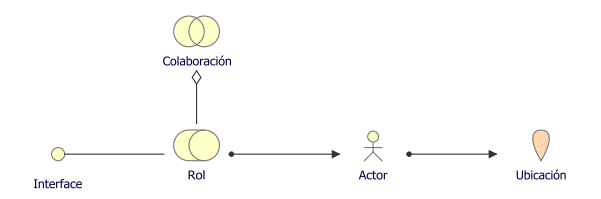
\includegraphics[width=0.8\linewidth]{development/organizacion.png}
			\caption{Metamodelo de Organización}
		\end{figure}
	
		\textbf{Caso}\\
		xxxxxxxxx\\
		
		\begin{figure}[H]
			\centering
			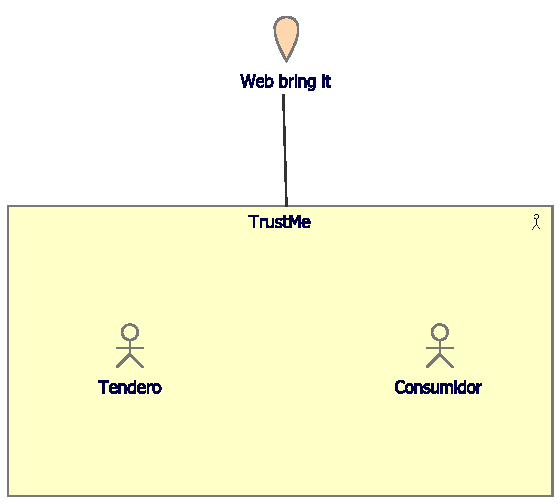
\includegraphics[width=0.8\linewidth]{development/negocio.pdf}
			\caption{Organización}
		\end{figure}
	}
	
	\subsection{Punto de vista de cooperación de actor}
	{ xxxxx\\
		
		\textbf{Modelo}\\
		\begin{figure}[H]
			\centering
			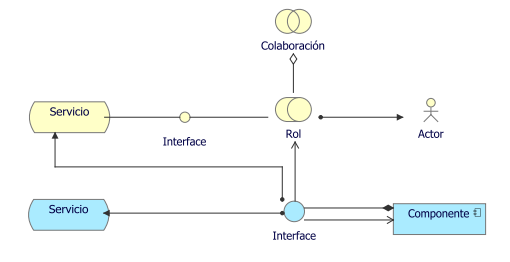
\includegraphics[width=0.8\linewidth]{development/cooperacionactor.png}
			\caption{Metamodelo de cooperación de actor}
		\end{figure}
		
		\textbf{Caso}\\
		xxxxxxxxx\\
		
		\begin{figure}[H]
			\centering
			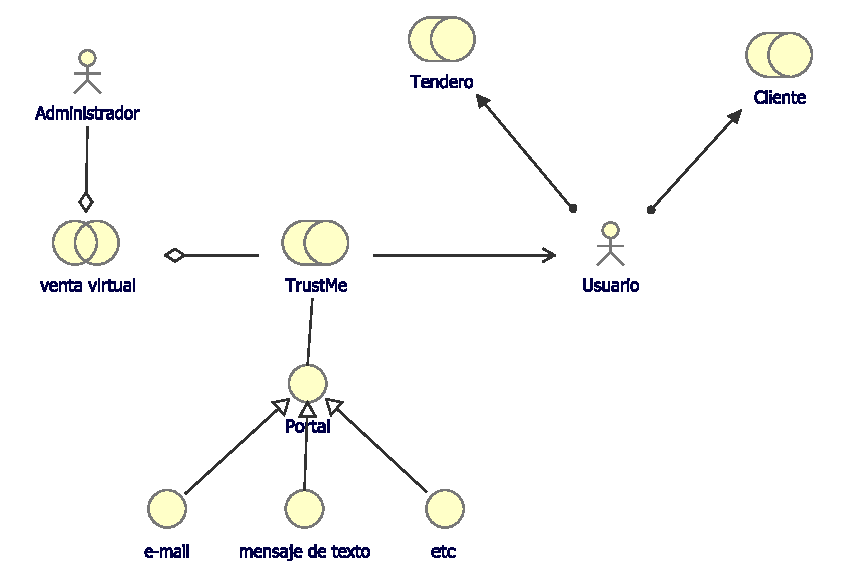
\includegraphics[width=0.8\linewidth]{development/cooperacionactor.pdf}
			\caption{Cooperación de actor}
		\end{figure}
	}
	
	\subsection{Punto de vista de función de negocio}
	{ xxxxx\\
		
		\textbf{Modelo}\\
		\begin{figure}[H]
			\centering
			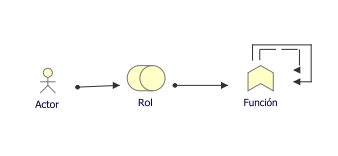
\includegraphics[width=0.8\linewidth]{development/funcion.png}
			\caption{Metamodelo de función de negocio}
		\end{figure}
		
		\textbf{Caso}\\
		xxxxxxxxx\\
		
		\begin{figure}[H]
			\centering
			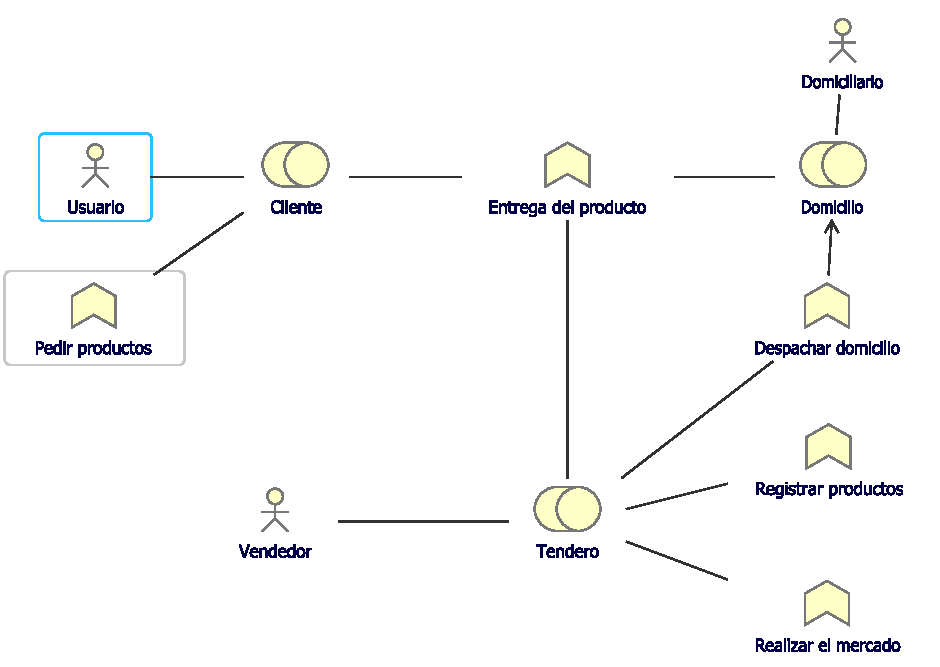
\includegraphics[width=0.8\linewidth]{development/funcion.pdf}
			\caption{Función de negocio}
		\end{figure}
	}
	
	\subsection{Punto de vista de proceso de negocio}
	{ xxxxx\\
		
		\textbf{Modelo}\\
		\begin{figure}[H]
			\centering
			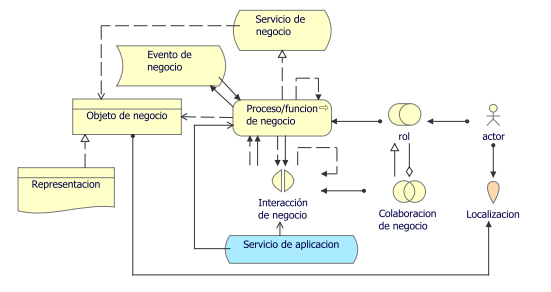
\includegraphics[width=0.8\linewidth]{development/proceso.png}
			\caption{Metamodelo de proceso de negocio}
		\end{figure}
		
		\textbf{Caso}\\
		xxxxxxxxx\\
		
		\begin{figure}[H]
			\centering
			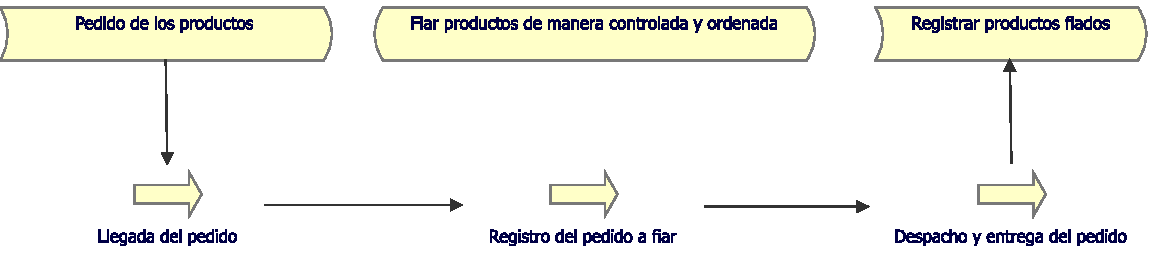
\includegraphics[width=0.8\linewidth]{development/proceso.pdf}
			\caption{Proceso de negocio}
		\end{figure}
	}
	
	\subsection{Cooperación de proceso de negocio}
	{ xxxxx\\
		
		\textbf{Modelo}\\
		\begin{figure}[H]
			\centering
			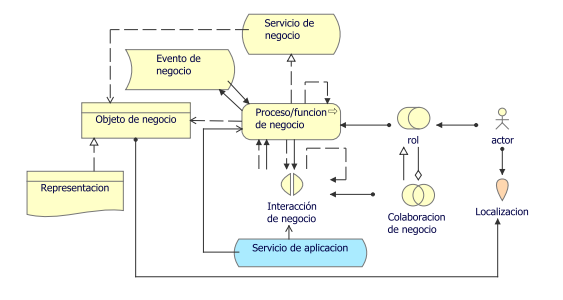
\includegraphics[width=0.8\linewidth]{development/cooperacionproceso.png}
			\caption{Metamodelo de cooperación de proceso de negocio}
		\end{figure}
		
		\textbf{Caso}\\
		xxxxxxxxx\\
		
		\begin{figure}[H]
			\centering
			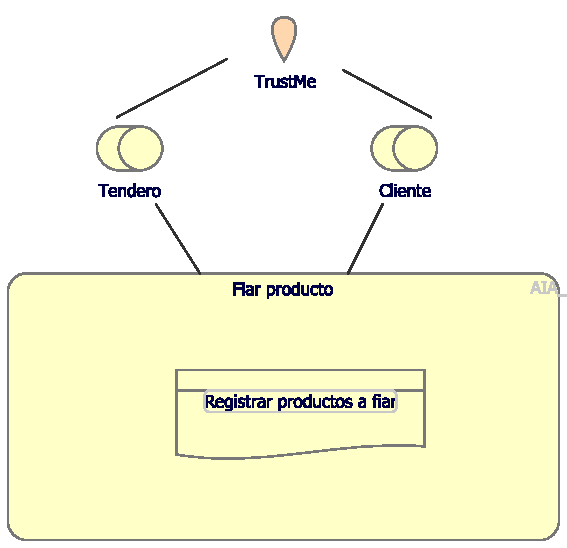
\includegraphics[width=0.8\linewidth]{development/cooperacionproceso.pdf}
			\caption{Cooperación de proceso de negocio}
		\end{figure}
	}
	
	\subsection{Punto de vista de producto}
	{ xxxxx\\
		
		\textbf{Modelo}\\
		\begin{figure}[H]
			\centering
			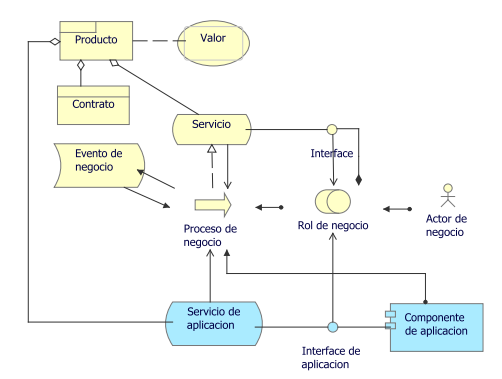
\includegraphics[width=0.8\linewidth]{development/producto.png}
			\caption{Metamodelo de producto}
		\end{figure}
		
		\textbf{Caso}\\
		xxxxxxxxx\\
		
		\begin{figure}[H]
			\centering
			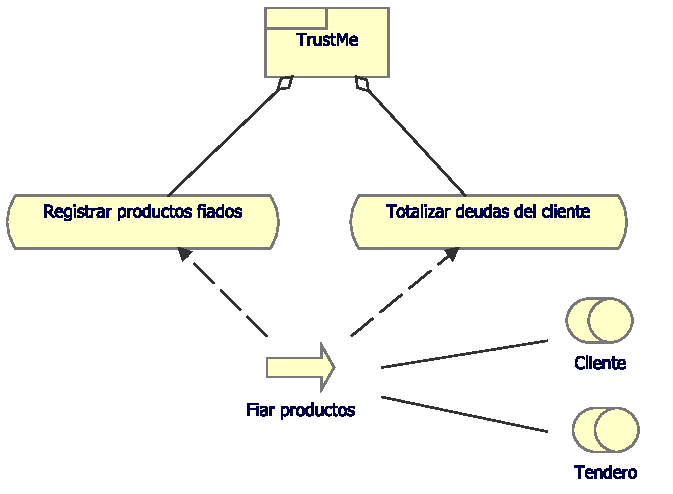
\includegraphics[width=0.8\linewidth]{development/producto.pdf}
			\caption{Producto}
		\end{figure}
	}
			\section{Arquitectura capa de aplicación}
{Esta capa, es la capa de arquitectura del proyecto orientada al aplicación, aquí se plasma la estructura de la aplicación del software soportado en componentes reusables e interfaces de comunicación.}

	\subsection{Punto de vista de comportamiento de aplicación}
	{ El comportamiento de aplicación muestra cómo se componen internamente una aplicación, es útil para diseñar el comportamiento principal del sistema o componentes, e identificar la superposición funcional de estas.\\
		
		\textbf{Modelo}\\
		\begin{figure}[H]
			\centering
			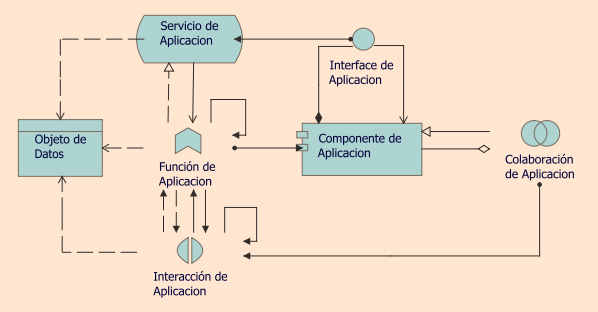
\includegraphics[width=0.8\linewidth]{development/comportamientoapp.png}
			\caption{Metamodelo Comportamiento de Aplicación}
		\end{figure}
	
		\textbf{Caso:} Los componentes de aplicación son:
		
		\begin{itemize}
			\item Gestionar préstamo
			\item Realizar préstamo
			\item Registrar usuarios
		\end{itemize}
		
		\begin{figure}[H]
			\centering
			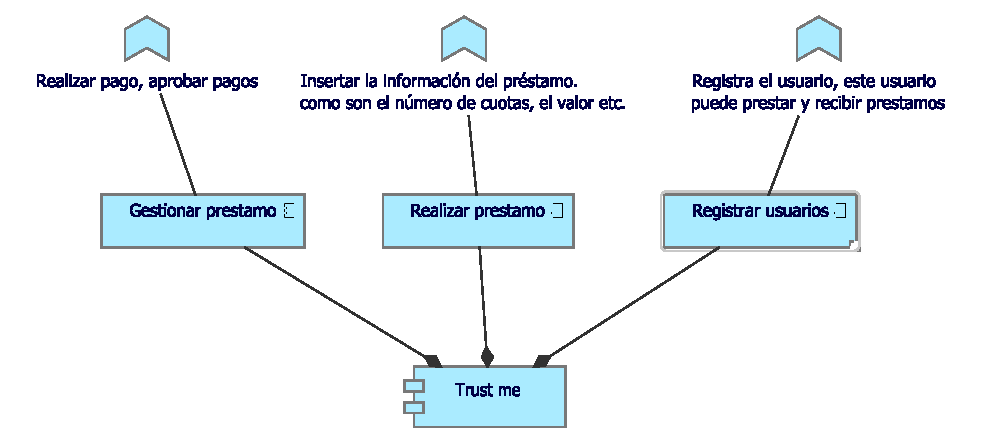
\includegraphics[width=0.6\linewidth]{development/comportamientoapp.pdf}
			\caption{Comportamiento de Aplicación}
		\end{figure}
	}
	
	\subsection{Punto de vista de cooperación de aplicación}
	{La  cooperación de aplicación describe las relaciones entre los componentes en términos de flujo de información o en términos de los servicios que estos proveen o usan. Este punto de vista también es usado para expresar la cooperación interna u orquestación de servicios que juntos soportan la ejecución de un proceso de negocio.\\
		
		\textbf{Modelo}\\
		\begin{figure}[H]
			\centering
			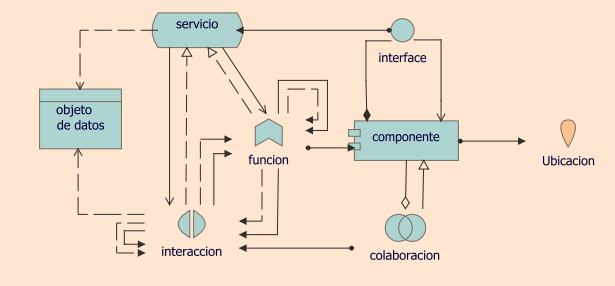
\includegraphics[width=0.8\linewidth]{development/cooperacionapp.png}
			\caption{Metamodelo Cooperación de Aplicación}
		\end{figure}
		
		\textbf{Caso:} 
		
		\begin{figure}[H]
			\centering
			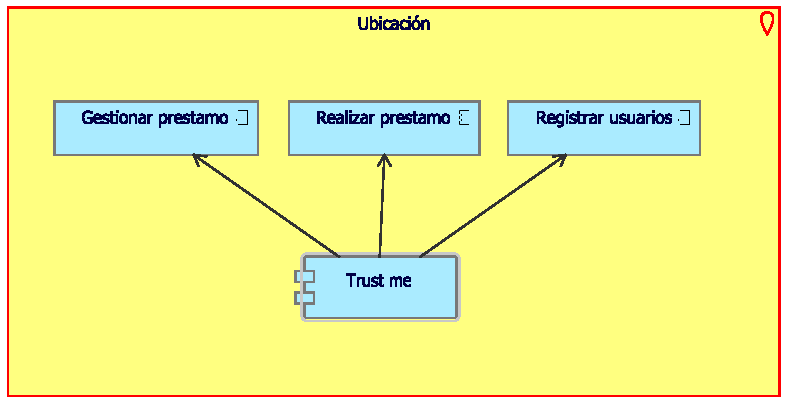
\includegraphics[width=0.8\linewidth]{development/cooperacionapp.pdf}
			\caption{Cooperación de Aplicación}
		\end{figure}
	}
	
	\subsection{Punto de vista de uso de aplicación}
	{
		
		\textbf{Modelo}\\
		\begin{figure}[H]
			\centering
			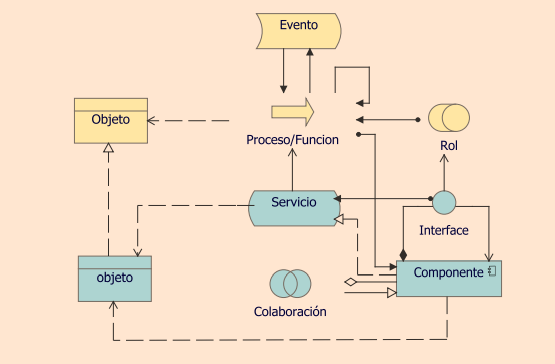
\includegraphics[width=0.8\linewidth]{development/usoapp.png}
			\caption{Metamodelo de Uso Aplicación}
		\end{figure}
		
		
		\begin{figure}[H]
			\centering
			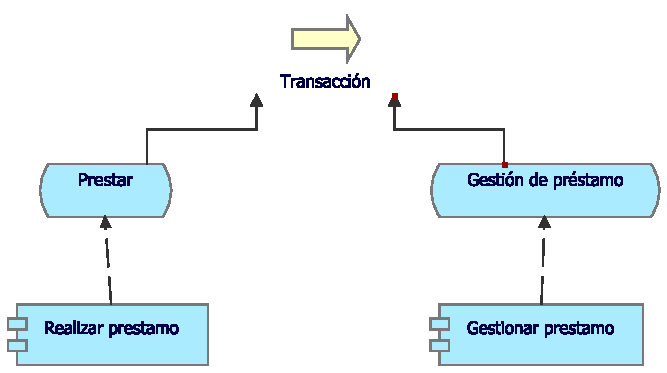
\includegraphics[width=0.8\linewidth]{development/usoapp.pdf}
			\caption{Uso Aplicación}
		\end{figure}
	}
	

			\section{Arquitectura capa de tecnología}

	\subsection{Punto de vista de infraestructura}
	{ 
		
		\textbf{Modelo}\\
		\begin{figure}[H]
			\centering
			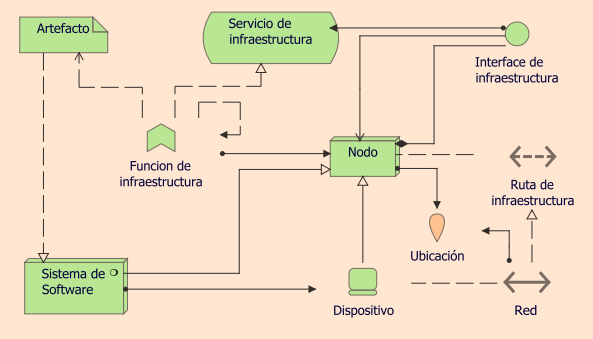
\includegraphics[width=0.8\linewidth]{development/infraestructura.png}
			\caption{Metamodelo de Infraestructura}
		\end{figure}
	
		\textbf{Caso:}
		
		\begin{figure}[H]
			\centering
			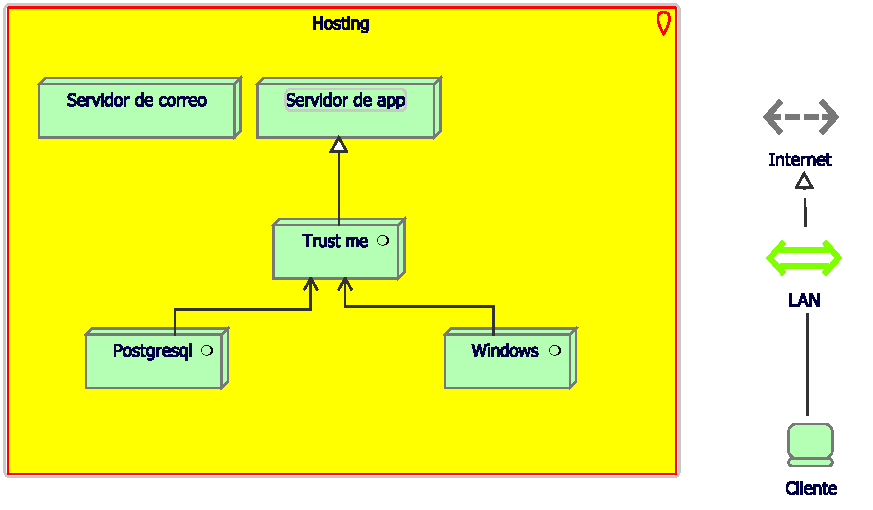
\includegraphics[width=0.6\linewidth]{development/infraestructura.pdf}
			\caption{Infraestructura}
		\end{figure}
	}
	
	\subsection{Punto de vista de uso de infraestructura}
	{
		
		\textbf{Modelo}\\
		\begin{figure}[H]
			\centering
			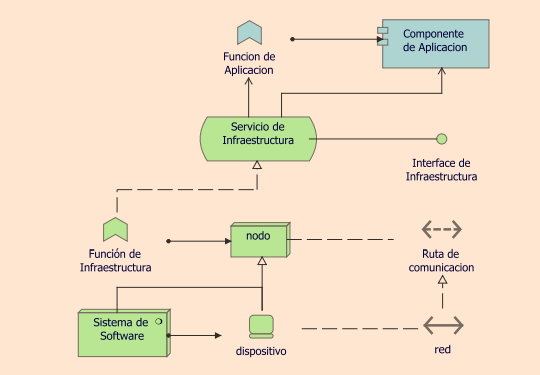
\includegraphics[width=0.8\linewidth]{development/usoinfraestructura.png}
			\caption{Metamodelo de Uso de Infraestructura}
		\end{figure}
		
		\textbf{Caso:} 
		
		\begin{figure}[H]
			\centering
			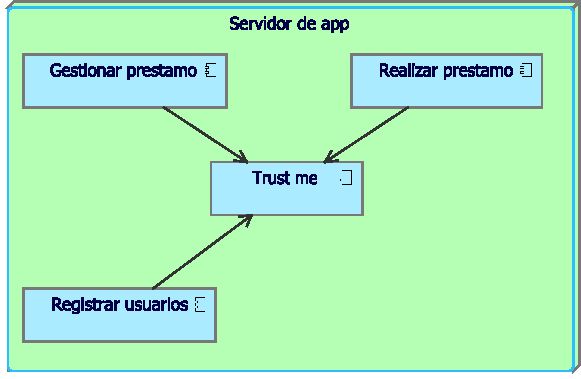
\includegraphics[width=0.8\linewidth]{development/usoinfraestructura.pdf}
			\caption{Uso de Infraestructura}
		\end{figure}
	}
	
	\subsection{Punto de vista de estructura de información}
	{		
		\textbf{Modelo}\\
		\begin{figure}[H]
			\centering
			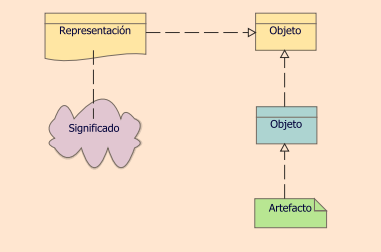
\includegraphics[width=0.8\linewidth]{development/estructurainfo.png}
			\caption{Metamodelo de Estructura de la información}
		\end{figure}
		
		\textbf{Caso:} 
		
		\begin{figure}[H]
			\centering
			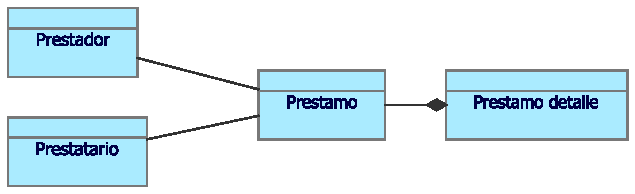
\includegraphics[width=0.8\linewidth]{development/estructurainfo.pdf}
			\caption{Estructura de la información}
		\end{figure}
	}
	
	\subsection{Punto de vista de realización del servicio}
	{ 		
		\textbf{Modelo}\\
		\begin{figure}[H]
			\centering
			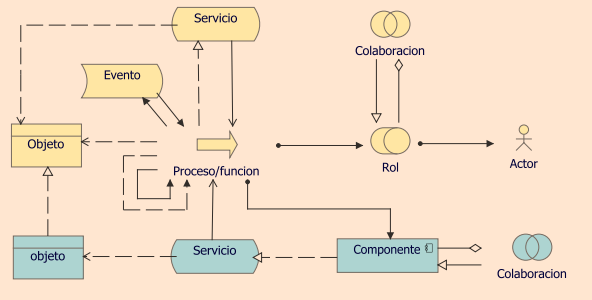
\includegraphics[width=0.8\linewidth]{development/realizacionser.png}
			\caption{Metamodelo de Realización Servicio}
		\end{figure}
		
		\textbf{Caso:}
			
		
		\begin{figure}[H]
			\centering
			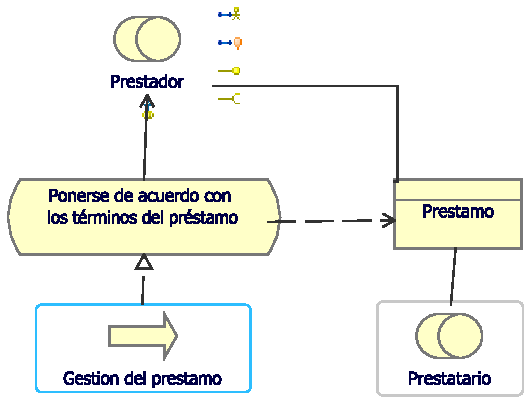
\includegraphics[width=0.8\linewidth]{development/realizacionser.pdf}
			\caption{Realización Servicio}
		\end{figure}
	}
	


	\part{CIERRE DE LA INVESTIGACIÓN}

		\chapter*{RESULTADOS Y DISCUSIÓN}
		\addcontentsline{toc}{chapter}{RESULTADOS Y DISCUSIÓN}
			\begin{itemize}
	\item Resultado 1.
	\item Resultado 2.
	\item Resultado 3.
\end{itemize}

		\chapter*{CONCLUSIONES}
		\addcontentsline{toc}{chapter}{CONCLUSIONES}
			\begin{itemize}
	\item Conclusion 1.
	\item Conclusion 2.
	\item Conclusion 3.
\end{itemize}
			\section{Aportes Originales}

	\begin{itemize}
		
		\item Creación de un modelo empresarial donde se gestione los prestamos de los tenderos hacia sus consumidores.
		
		\item Permitir el acceso de personas de bajos recursos a productos de bajo costo, por medio de la tecnología.
		
		\item Procesar las apuestas informales o deudas entre conocidos, para tener un mejor control de estas.
		
	\end{itemize}
			\section{Trabajos o publicaciones derivadas}
	{El modelo de negocio planteado, puede derivar en la creación propia de cada tendero de su sitio WEB, donde procese los pagos de sus clientes y obtener un control o dominio total, de lo que se acontece en su negocio.}
			
		\chapter*{PROSPECTIVA DEL TRABAJO DE GRADO}
		\addcontentsline{toc}{chapter}{PROSPECTIVA DEL TRABAJO DE GRADO}
			\section{Trabajos de investigación futuros}

	{A futuro, se propone implementar lo siguiente:
		
	\begin{itemize}
		\item Una integración con centros de pagos, que permitan procesar el pago online de sus deudas con sus respectivos prestamistas y así, evitar el manejo de efectivo, acercando un poco más la plataforma a las últimas tendencias tecnológicas de los usuarios.
		
		\item Una arquitectura de software mantenible y desacoplada por medio de microservicios, que permita la integración vía API con varias tecnologías, como lo es Android, IPhone, Mac, Windows etc. Posibilitando el renderizado de vistas según la información suministrada por el microservicio, utilizando cualquier lenguaje de programación.
	\end{itemize}
		
	Por otro lado, se pretende ampliar el modelo de negocio propuesto, donde se permita abarcar almacenes de cadena que accedan a este tipo de actividad económica, posibilitando un ingreso económico extra.
	}
\clearpage
			
	\renewcommand{\bibname}{REFERENCIAS}	
	\bibliographystyle{ieeetr}
	\addcontentsline{toc}{part}{REFERENCIAS}
	\bibliography{bibliography/articles,bibliography/books,bibliography/online}
	
	\chapter*{ANEXOS}
	\addcontentsline{toc}{part}{ANEXOS}
		\section*{Anexo A. Recolección de la información}
\addcontentsline{toc}{section}{Anexo A. Recolección de la información}

	\subsection*{Encuesta}
	\addcontentsline{toc}{subsection}{Encuesta}
	
	{Para obtener la información base para el desarrollo del proyecto, fue indispensable utilizar la técnica de recolección de información “encuesta”, donde se plasmaron las inquietudes que permitieron estructurar adecuadamente el proyecto.\\
		
	La encuesta realizada fue la siguiente (se utilizó la plataforma Formularios de Google para publicar y obtener los resultados de esta):
	
	\begin{enumerate}
		
		\item ¿Ha recurrido el sistema de “fiado” que utilizan algunos tenderos para adquirir productos?
		
			\begin{enumerate}
				\item Si.
				\item No.
			\end{enumerate}
		
		\item ¿Ha tenido problemas al momento de pagar sus productos fiados, ya que el monto de la deuda es mayor o menor al que tenía en mente?
		
			\begin{enumerate}
				\item Si.
				\item No.
			\end{enumerate}	
		
		\item Cuándo realiza un préstamo, ¿dónde realiza el registro de este, para su posterior control?
			
			\begin{enumerate}
				\item Tomo notas en el celular.
				\item Tomo notas en cuadernos o agendas.
				\item No tomo notas.
				\item Otro.
			\end{enumerate}
		
		\item ¿Suele olvidarse de las deudas que tienen algunas personas con usted (personas de confianza)?
		
			\begin{enumerate}
				\item Si.
				\item No.
			\end{enumerate}	
		
		\item Considera que utilizar una plataforma Web que permita gestionar los fiados y prestamos es:
		
			\begin{enumerate}
				\item Pertinente.
				\item Innecesaria.
			\end{enumerate}
		
	\end{enumerate}
	}
	

	
	

\end{document}          
